\chapter{Analysis of SMELLIE Data in the Scintillator Phase}\label{chap:smellie_analysis}
% \epigraph{\textit{}}{source}

This chapter contains two sets of analyses: measurements of the extinction lengths of the scintillator as a function of wavelength and time, as well as monitoring the Rayleigh scattering length over time. In both cases, care had to be taken to try and make the methodologies robust to systematics.

\section{Extinction Length Analysis}\label{sec:ext_length_analysis}
% \subsection{Motivation}
% \begin{itemize}
%     \item Explain motivating observations for this analysis: a substantial discrepancy between MC and data seen in the radial profiles of nhitsCleaned for \ce{^{210}Po} after the PPO top-up campaign. Performed by Serena.
%     \item Hypothesis of a shortening of the absorption/scattering length proposed, further strengthened by Ben Tam's ex-situ absorption measurements with scintillator taken from the detector, as well as knowledge about a likely ``cooking'' of PPO during the PPO-fill.
%     \item Describe the provisional optics model decided on based on these measurements, which includes an additional non-re-emitting component of the scintillator.
%     \item As a further cross-check, SMELLIE should be sensitive to changes in the overall extinction length of the scintillator, especially for short extinction lengths relative to the size of the detector.
%     \item More straightforward in measuring extinction length compared to scattering length --- no need to distinguish between scintillator re-emission and scattering.
%     \item Further uses: can be used to monitor the extinction length over time!
% \end{itemize}
% [4 pages]
The first analysis discussed in this chapter is the measurement of the extinction lengths of the liquid scintillator deployed in the SNO+ detector, as a function of both wavelength and time. As seen in Fig.~\ref{fig:smellie_timeline}, SMELLIE data was taken during the water phase, and in the scintillator phase when the PPO concentration of the LABPPO was at a variety of levels. Fig.~\ref{fig:smellie_expected_ext_length_phases} shows the expected changes in extinction length with detector phase, as a function of wavelength, according to the optical model described in Section~\ref{sec:optical_processes}.

\begin{figure}
    \centering
    % 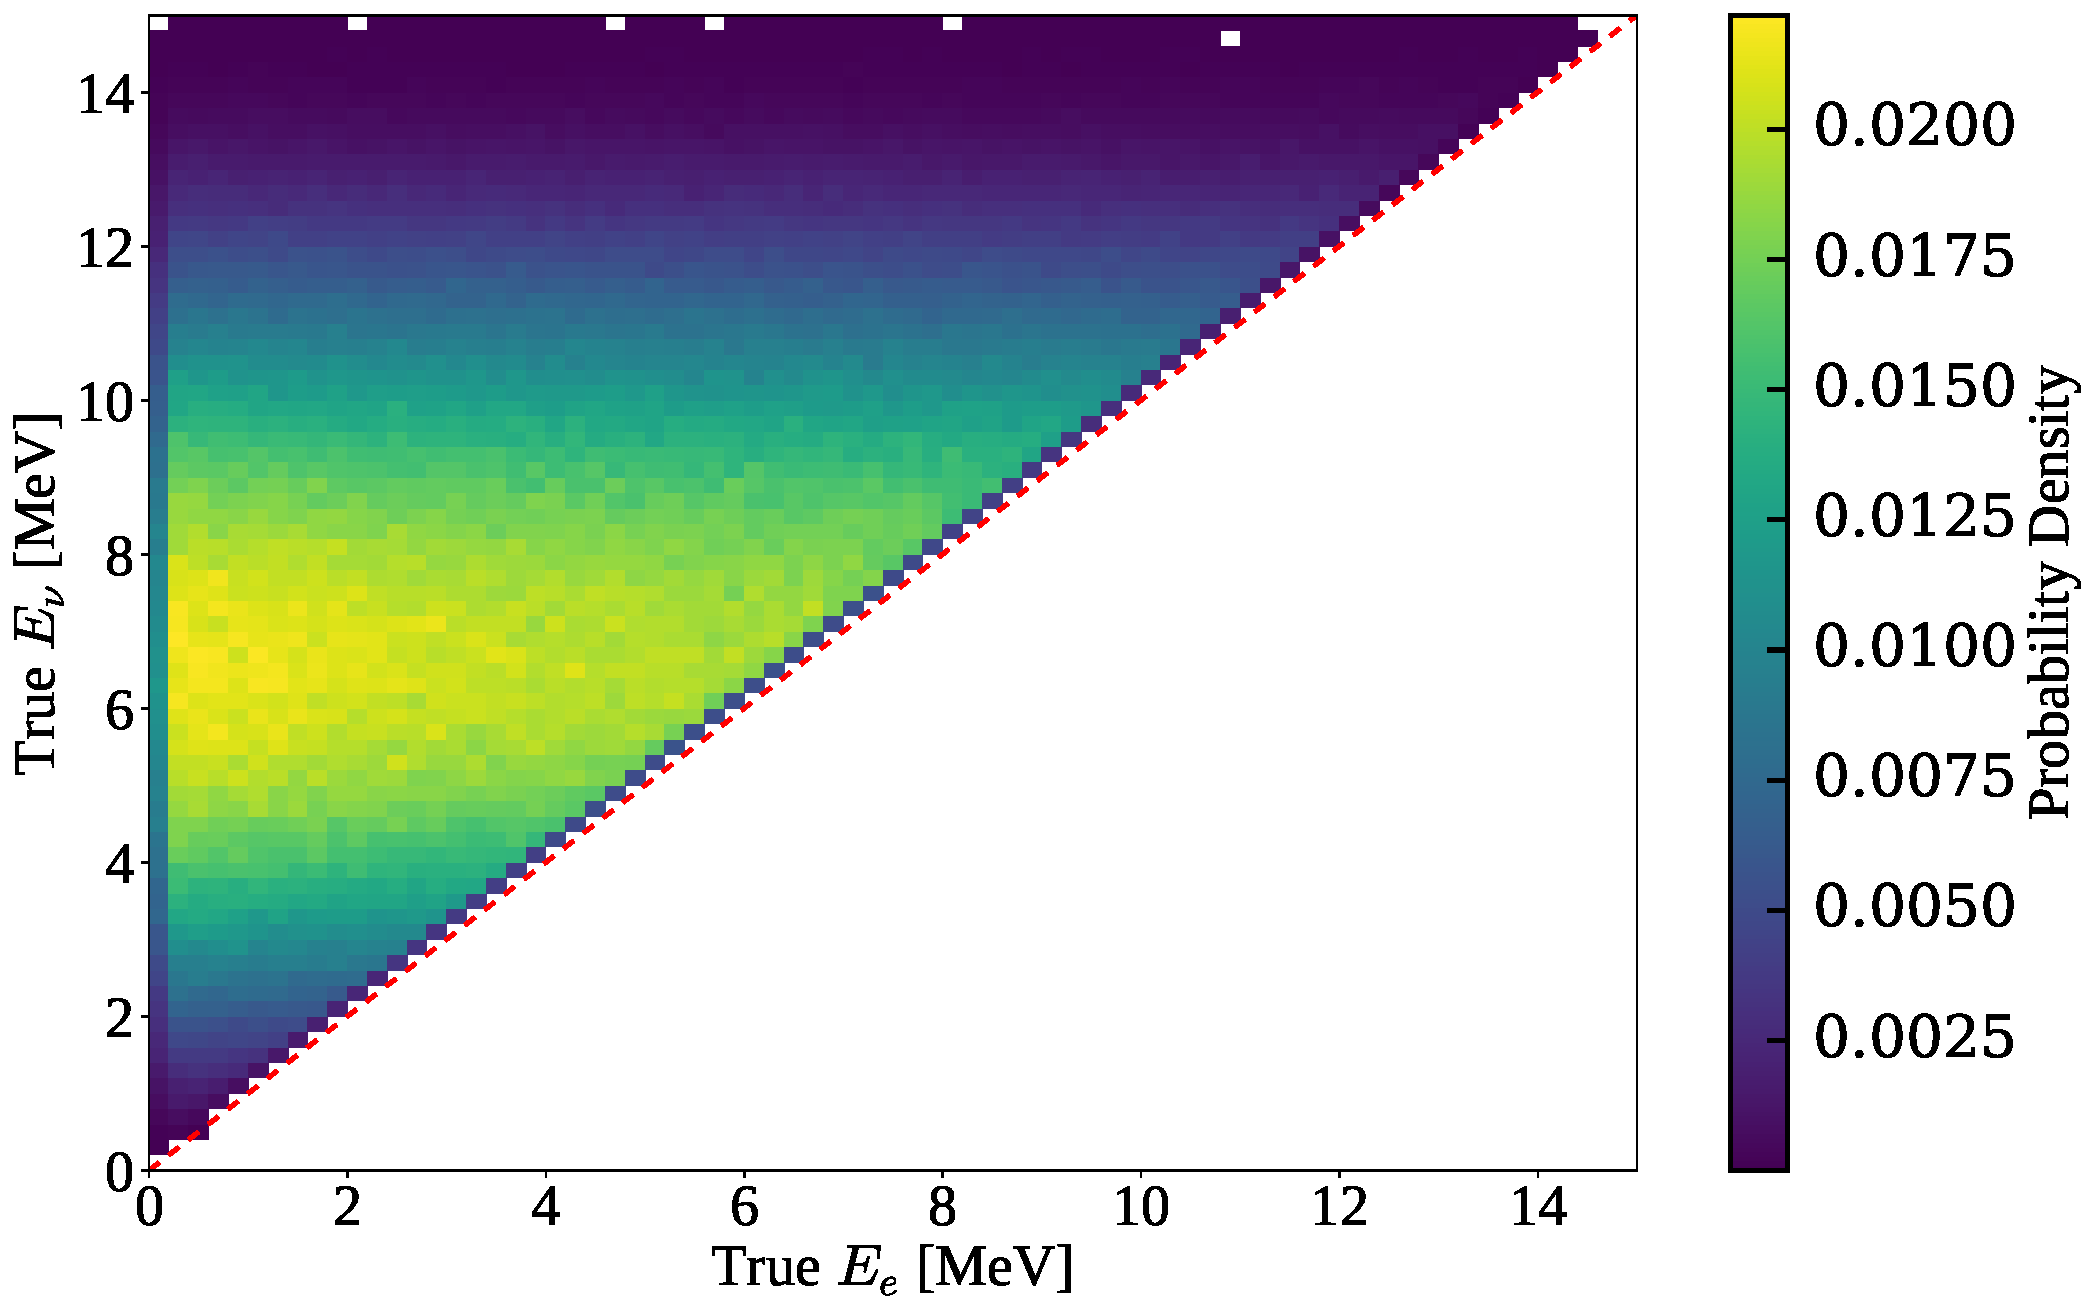
\includegraphics[width=0.8\textwidth]{6_SolarAnalysis/images/b8_eelectrue_vs_enutrue.pdf}
    \caption[]{}
    \label{fig:smellie_expected_ext_length_phases}
\end{figure}

\subsection{Analysis Approach}
\subsubsection{The 2-PMT Case}
To begin, consider light emission from a particular SMELLIE fibre of fixed wavelength $\lambda_{j}$, with a mean emission intensity of $I_{j}$ photons emitted per event in subrun $j$ during detector phase $p$. Modifying Eq.~\ref{eq:mu_def}, a general PMT $i$ will have a mean npe per event of $\mu_{ij,p}(\lambda_{j}) = I_{j,p}b_{i,p}(\lambda_{j})f_{i,p}(\lambda_{j})$. A detector phase-dependence has been added to all terms, because:
\begin{itemize}
    \item The emission intensities chosen, $I_{j,p}$, can vary between different data-taking campaigns. These changes are due to changes in hardware (as detailed in Chapter~\ref{chap:smellie_hardware}), as well as changes in the settings used to run SMELLIE.
    \item The beam profile of a given fibre at a given wavelength is not expected to change with detector phase. However, if the refractive index of the inner detector medium changes (e.g. from the water phase to scintillator phase), then the fraction of light emitted that is pointed in the correct direction to be detected by PMT $i$, $b_{i,p}(\lambda_{j})$, \textit{can} change. This effect is discussed in more detail in Section~\ref{sec:smellie_ext_corrections}.
    \item In a different phase of the detector, the optics of the inner detector can certainly change, and so the probability that a photon pointing in the correct direction for PMT $i$ actually makes it across the detector and generates a photoelectron, $f_{i,p}(\lambda_{j})$, can change.
\end{itemize}

For the purposes of this analysis, consider specifically PMTs in the beamspot of the fibre with unobstructed paths. Then, a given beamspot PMT will have a mean npe per event, $\mu_{ij,p}^{\mathrm{beam}}(\lambda_{j})$, of:
\begin{align}\label{eq:smellie_ext_length_theory}
    \mu_{ij,p}^{\mathrm{beam}}(\lambda_{j}) &= I_{j,p}b_{i,p}(\lambda_{j})
    \exp\left(
        -\frac{L_{ij,p}^{\mathrm{extern}}(\lambda_{j})}{l^{\mathrm{extern}}(\lambda_{j})}
    \right)
    \exp\left(
        -\frac{L_{ij,p}^{\mathrm{acr}}(\lambda_{j})}{l^{\mathrm{acr}}(\lambda_{j})}
    \right)
    \exp\left(
        -\frac{L_{ij,p}^{\mathrm{inner}}(\lambda_{j})}{l_{p}^{\mathrm{inner}}(\lambda_{j})}
    \right)\nonumber\\
    & \qquad\cdot T_{ij,p}(\lambda_{j})\epsilon_{ij,p}(\lambda_{j}).
\end{align}
Here, $L_{ij,p}^{\mathrm{extern,acr,inner}}(\lambda_{j})$ is the length of a path in a given detector medium through which light travels, for the external water, acrylic, and inner detector medium, respectively. $l_{p}^{\mathrm{extern,acr,inner}}(\lambda_{j})$ is the extinction length of each detector medium for a given wavelength --- it is assumed that only the inner detector medium has changing optics in different phases. Some fraction of light is lost when passing between two mediums with different refractive indices: this is captured by $T_{ij,p}(\lambda_{j})$, the product of the Fresnel transmission components for all optical boundaries along a photon's path. Finally, $\epsilon_{ij,p}(\lambda_{j})$ is the probability that a photon along a given path, incident on a given PMT, will generate a photoelectron that is detected. 

Measuring $l_{p}^{\mathrm{inner}}(\lambda_{j})$ is the aim of this analysis. In order to do so, all other parameters in Eq.~\ref{eq:smellie_ext_length_theory} must either be measured, or removed in some careful way. As discussed in Section~\ref{sec:optical_processes}, the extinction lengths of both the UPW and the acrylic were measured as a function of wavelength in the water phase with the Laserball. It is assumed that the optics of the UPW inside and outside the AV were the same, and have not changed since. That section also discusses the measured refractive indices as a function of wavelength for the UPW, acrylic, and LABPPO. For a given detector phase, subrun, and PMT, the Collaboration's \texttt{Light Path Calculator} is able to determine the values of $L_{ij,p}^{\mathrm{extern,acr,inner}}(\lambda_{j})$ as well as the combined Fresnel transmission coefficient $T_{ij,p}(\lambda_{j})$.

As will be discussed in Section~\ref{sec:smellie_intensity}, measuring the absolute value of $I_{j,p}$ is challenging. Fortunately, there are ways of making relative intensity calibrations, which is sufficient for this analysis. Consider PMTs near the fibre emission point. The first light observed by these PMTs will be from photons which have `back-scattered' off of the UPW outside the AV. This is followed by light reflected off of the AV surface. Fig.~\ref{fig:smellie_back_PMTs_tres_plot} shows the observed time residual distribution for such a PMT. As can be seen, the back-scattered light is well-separated in time from all other optical processes. Assuming that the Rayleigh scattering properties of the UPW outside the AV have been unchanged throughout the lifetime of the detector, then the expected number of photoelectrons observed in a selection of these PMTs during a time period in which only back-scattering can occur will be simply:
\begin{equation}
    \mu_{j,p}^{\mathrm{back}} = kI_{j,p}.
\end{equation}
$k$ here is just some general constant of proportionality.

\begin{figure}
    \centering
    % 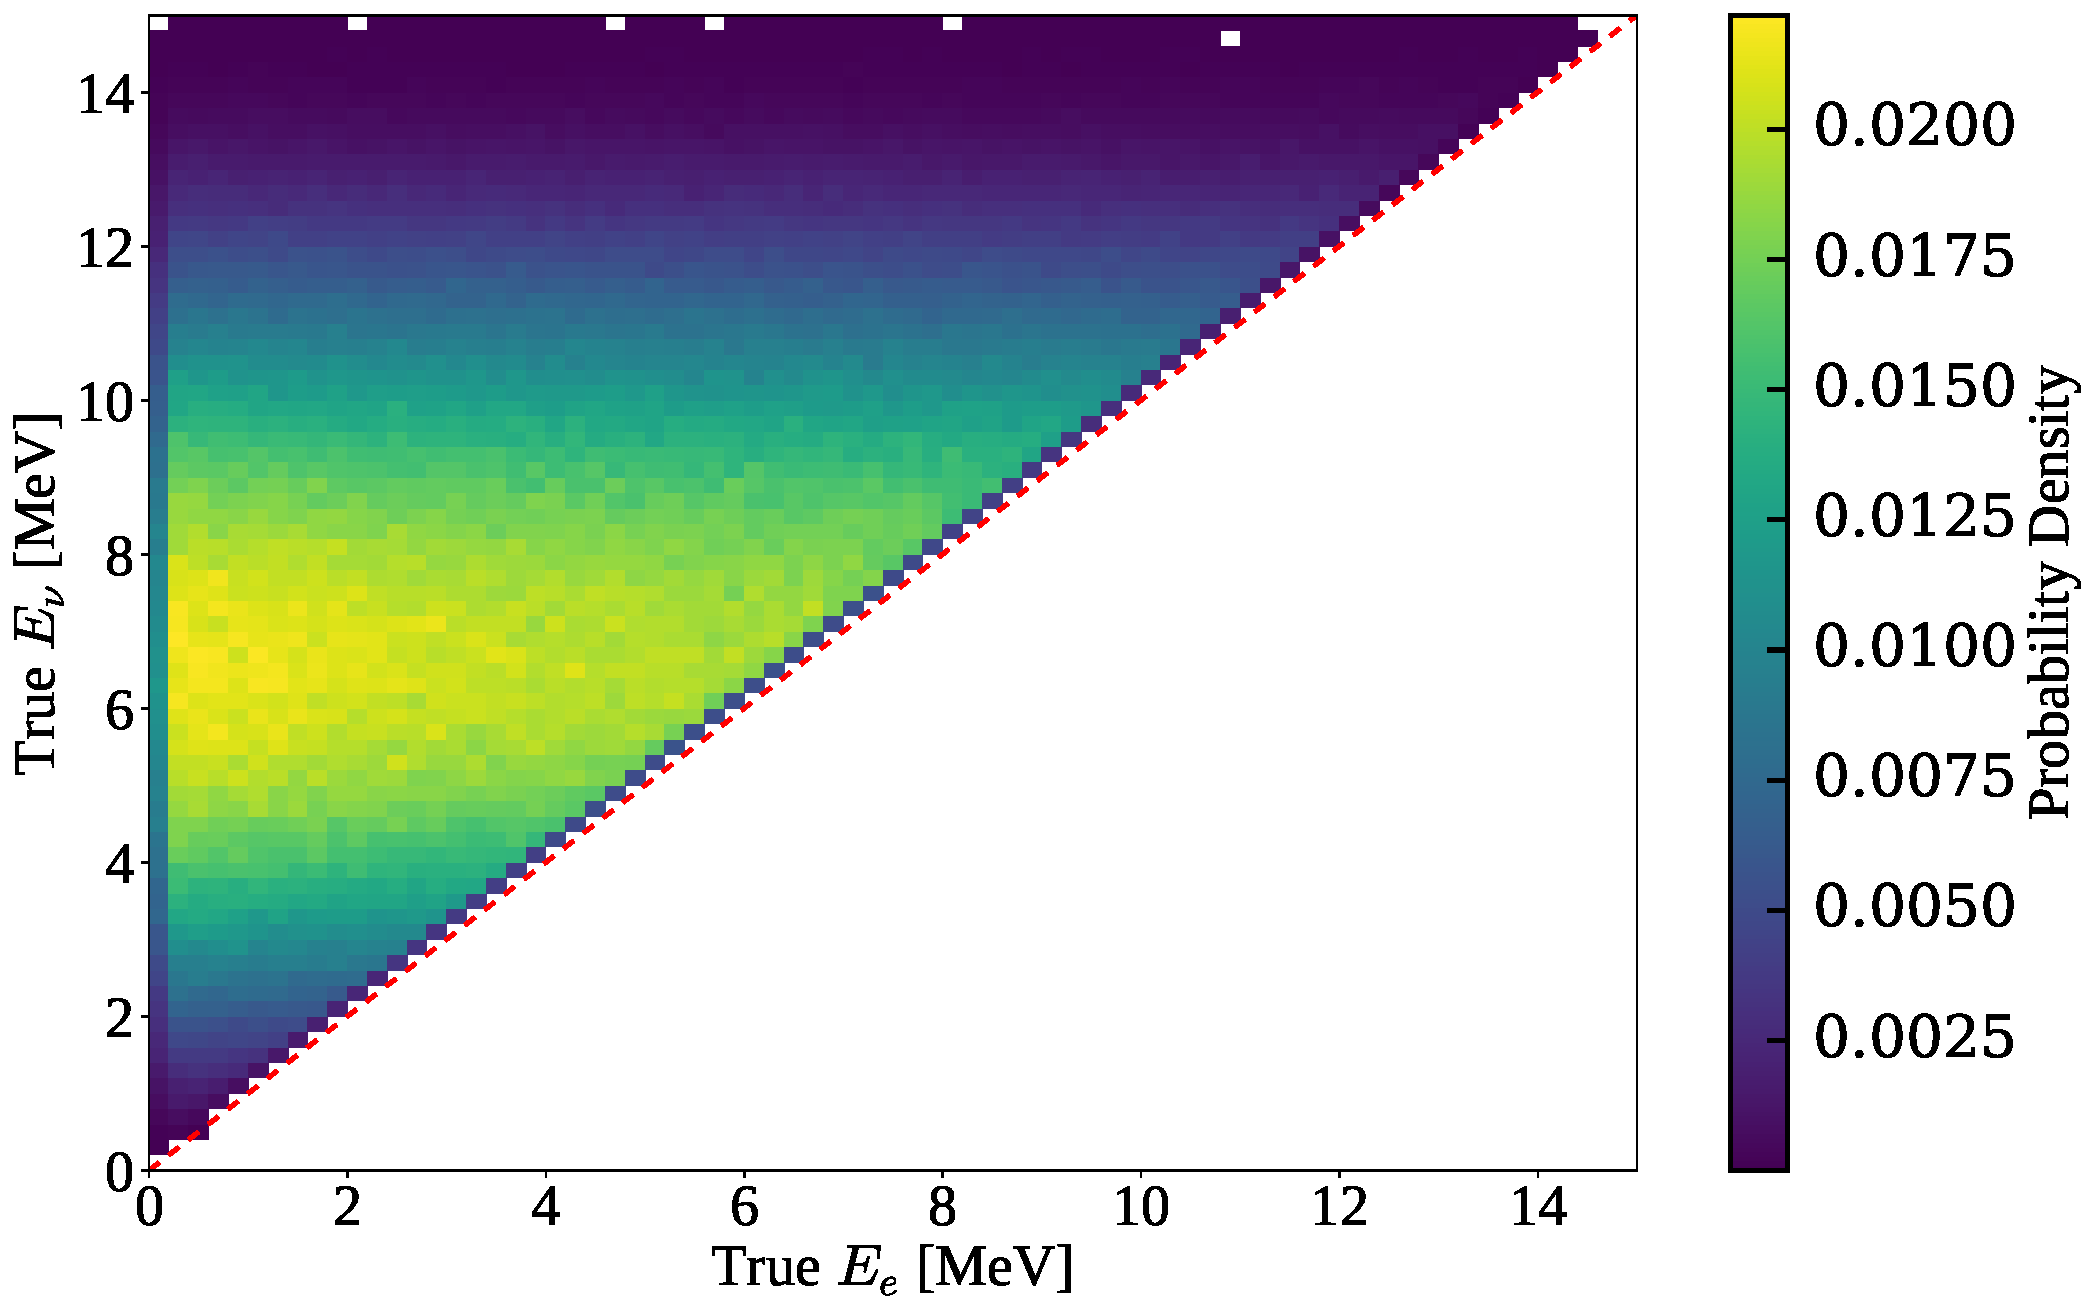
\includegraphics[width=0.8\textwidth]{6_SolarAnalysis/images/b8_eelectrue_vs_enutrue.pdf}
    \caption[]{}
    \label{fig:smellie_back_PMTs_tres_plot}
\end{figure}

Because $\mu_{j,p}^{\mathrm{back}}$ is proportional to the intensity, the ratio $R_{ij,p} = \mu_{ij,p}^{\mathrm{beam}}(\lambda_{j})/\mu_{j,p}^{\mathrm{back}}$ will be independent of $I_{j,p}$. A similar trick can be used to remove the dependence of $R_{ij,p}$ on $k$, by taking the ratio of $R_{ij,p}$ with $R_{ij,\ce{H_{2}O}}$, where $R_{ij,\ce{H_{2}O}}$ is the measured values of $R_{ij,p}$ in the water phase. This ratio becomes:
\begin{align}
    \frac{R_{ij,p}}{R_{ij,\ce{H_{2}O}}}(\lambda_{j}) 
    &= \frac{k}{k}
    \frac{b_{i,p}(\lambda_{j})}{b_{i,\ce{H_{2}O}}(\lambda_{j})}
    \frac{T_{ij,p}(\lambda_{j})}{T_{ij,\ce{H_{2}O}}(\lambda_{j})}
    \frac{\epsilon_{ij,p}(\lambda_{j})}{\epsilon_{ij,\ce{H_{2}O}}(\lambda_{j})}
    \exp\left(
        -\frac{L_{ij,p}^{\mathrm{extern}}(\lambda_{j})-L_{ij,\ce{H_{2}O}}^{\mathrm{extern}}(\lambda_{j})}{l^{\mathrm{extern}}(\lambda_{j})}
    \right)
    \nonumber\\
    & \quad \cdot \exp\left(
        -\frac{L_{ij,p}^{\mathrm{acr}}(\lambda_{j})-L_{ij,\ce{H_{2}O}}^{\mathrm{acr}}(\lambda_{j})}{l^{\mathrm{acr}}(\lambda_{j})}
    \right)
    \exp\left(
        -\frac{L_{ij,p}^{\mathrm{inner}}(\lambda_{j})}{l_{p}^{\mathrm{inner}}(\lambda_{j})}
        +\frac{L_{ij,\ce{H_{2}O}}^{\mathrm{inner}}(\lambda_{j})}{l_{\ce{H_{2}O}}^{\mathrm{inner}}(\lambda_{j})}
    \right)
    \nonumber\\
    &= \frac{b_{i,p}(\lambda_{j})\epsilon_{ij,p}(\lambda_{j})}{b_{i,\ce{H_{2}O}}(\lambda_{j})\epsilon_{ij,\ce{H_{2}O}}(\lambda_{j})}
    \frac{T_{ij,p}(\lambda_{j})}{T_{ij,\ce{H_{2}O}}(\lambda_{j})}
    \exp\left(
        -\frac{L_{ij,p}^{\mathrm{inner}}(\lambda_{j})}{l_{p}^{\mathrm{inner}}(\lambda_{j})}
        +\frac{L_{ij,\ce{H_{2}O}}^{\mathrm{inner}}(\lambda_{j})}{l_{\ce{H_{2}O}}^{\mathrm{inner}}(\lambda_{j})}
    \right),
\end{align}
where it has been assumed that any change in path length through the external UPW or acrylic relative to their extinction lengths is negligible.

Rearranging the above for $l_{p}^{\mathrm{inner}}(\lambda_{j})$, one can write:
\begin{align}\label{eq:smellie_ext_length_1PMT}
    l_{p}^{\mathrm{inner}}(\lambda_{j}) &= 
    \frac{
        L_{ij,p}^{\mathrm{inner}}(\lambda_{j})
        }{
        \ln\left(
            \frac{R_{ij,\ce{H_{2}O}}}{R_{ij,p}}(\lambda_{j})\cdot s_{ij,p}(\lambda_{j})
        \right)
        + \ln\left(
            \frac{T_{ij,p}(\lambda_{j})}{T_{ij,\ce{H_{2}O}}(\lambda_{j})}
        \right)
        + \frac{L_{ij,\ce{H_{2}O}}^{\mathrm{inner}}(\lambda_{j})}{l_{\ce{H_{2}O}}^{\mathrm{inner}}(\lambda_{j})}
    },\nonumber\\
    s_{ij,p}(\lambda_{j}) &=
    \frac{
        b_{i,\ce{H_{2}O}}(\lambda_{j})\epsilon_{ij,\ce{H_{2}O}}(\lambda_{j})
        }{
        b_{i,p}(\lambda_{j})\epsilon_{ij,p}(\lambda_{j})
    }.
\end{align}
The parameter $s_{ij,p}(\lambda_{j})$ describes the fractional change in observed npe for a given PMT due to differences in refraction between the phases. Quantifying this effect will be discussed in Section~\ref{sec:smellie_ext_corrections}.


% \begin{itemize}
%     \item Outline theoretical approach for how one could measure the extinction length of scintillator through a comparison of SMELLIE data between the scintillator and water phases, in the simplified 1 dimensional case with only 2 PMTs.
% \end{itemize}
% [3 pages]

\subsubsection{Combining Results Between PMTs}
The formula described in Eq.~\ref{eq:smellie_ext_length_1PMT} is theoretically able to measure the extinction length of the liquid scintillator using one beamspot PMT and a number of `back-scatter' PMTs. Conveniently, numerous beamspot PMTs exist, which means each can be used to make a separate measurement of the extinction length, and then the measurements combined afterwards. One could alternatively consider the total npe detected in all beamspot PMTs together, but this wouldn't account for the different path lengths through the scintillator that light has to travel to get to different beamspot PMTs.



{
\color{blue}
\begin{itemize}
    \item Not doing analysis with just 2 PMTs, of course! Can combine results from multiple PMTs within a beamspot: I explain how here.
\end{itemize}
[2 pages]

\subsubsection{Corrections Between the Water and Scintillator Phases}\label{sec:smellie_ext_corrections}
\begin{itemize}
    \item Note the complications that we have to deal with. Namely, the differing refractive indices of the media bending the beamspot differently in the phases, as well as the method used to estimate $t_{\textrm{emm}}$.
    \item Explain how we deal with these, the former through MC simulation.
\end{itemize}
[2 pages]
\subsection{Validation of the Analysis in Simulation}
\begin{itemize}
    \item Show results of this approach being used to measure the extinction length in simulation. How well does it do?
\end{itemize}
[3 pages]
\subsection{Results in Data}
\begin{itemize}
    \item Describe the data used in this analysis, both water and scintillator, which can be shown in a table.
    \item Show examples of analysis of data in action for \SI{375}{\nm} data: typical $t_{\textrm{res}}$ distributions of backscattered and beamspot PMTs; calculation of that particular extinction length measurement, followed by the graph for extinction length in \SI{375}{\nm} over all fibres and time periods.
    \item Discuss what results can be seen in this plot: consistency between fibres, the expected change as a function of PPO concentration, and stability of the extinction length during the main \SI{2.2}{\gpl} scintillator phase.
    \item Compare results to those made by Ben ex-situ: are they in agreement? If not, what possible systematics could there be? The main one for my analysis is likely to be uncertainties in the simulated beam profile that leak through into the refractive index correction of the beamspot. For the ex-situ analysis, the value of the extinction length obtained is achieved through background subtraction at some long wavelength, and the particular choice of this wavelength can lead to systematic changes in the obtained extinction length.
    \item Look at results at longer wavelengths: can anything reasonably be said at these longer wavelengths? Why/why not?
    \item Finally: describe any conclusions that can be reached, in particular whether we can affirm the optics model we use in RAT.
\end{itemize}
[8 pages]

\section{Scattering Analysis}\label{sec:scattering_analysis}
\subsection{Historical Approaches and the Problem of Systematics}
\begin{itemize}
    \item Comparison to MC is necessary in scattering analysis, compared to merely being needed as a correction factor. This is because of the angular dependence of scattering. As a result, we can be far more susceptible to systematics from poor modelling!
    \item As a warning, show how Krish's/Esther's approach to the SMELLIE scattering analysis suffers majorly from these systematic effects. Requires describing their analysis approach briefly, and then explaining how the systematics described in Section~\ref{sec:smellie_systematics} lead to major problems with this approach.
    \item Motivates the need for either reduced systematics, or an alternative analysis approach that is more robust to them!
\end{itemize}
[2 pages]
\subsection{New Methodology}
\subsubsection{Signal Region Selection}
\begin{itemize}
    \item Propose the new analysis approach: looking at light in the ``bad light-path'' PMT region. Define what this region is.
    \item Give qualitative argument for why we expect this region to be robust to the beam profile systematics: dominated by the scattered signal as no direct light can make it here, and changes to beam profile should get ``smeared out'' after scattering.
    \item Show how simulations indicate this should be a region with a very high purity of scattered light, and (assuming all else being equal) robust to beam profile uncertainties.
    \item Confirm robustness of selected PMT region to uncertainties in AV offset and fibre position.
\end{itemize}
[5 pages]
\subsubsection{Measuring the Emission Intensity}\label{sec:smellie_intensity}
\begin{itemize}
    \item Remaining systematics is now in the calculation of an average absolute emission intensity.
    \item Show how various methods don't work particularly well: whole detector npe, beamspot npe, backscattered light npe, ``bad light-path'' PMTs but at later times. Explain why it goes wrong for each method.
    \item Look at "beamspot but excepting the central bit": if that works well, then we can continue!
    \item Otherwise, we'll have to live with measuring relative scattering lengths instead of absolute amounts, using the outer water back-scattering as a measure of the relative emission intensity.
\end{itemize}
[4 pages]
\subsection{Results}
\begin{itemize}
    \item Actually do the proposed analysis on data, versus time and wavelength. Do the results seem consistent between fibres? Are they sensible values?
\end{itemize}
[5 pages]
[33 PAGES TOTAL]
}